% !TEX root = deckblatt4.tex
\section{Messung eines Rechtecksignals}
\subsection{Aufgabenstellung}
Hier sollte ein Rechtecksignal in Zeit und Frequnenzbereich gemessen werden und anschlie\ss{}end die Ergebnisse erl\"autert werden

\subsection{Vorbereitung \& Messaufbau}
Es wurde mit dem Frequnezgenerator ein Rechtecksingal mit einer Amplitude von $1V_{pp}$ und einer Frequnez von $10kHz$ erzeugt. Der Ausgang des Frequnezgenerators wurde direkt mit dem Tastkopf des Oszilloskops verbunden, es wurde keine Messschaltung aufgebaud.

\begin{figure}[H]
 \begin{center}
  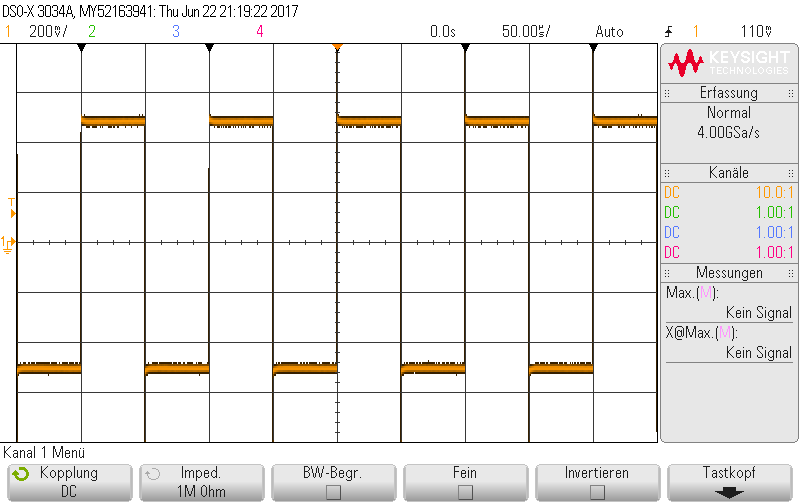
\includegraphics[height=6cm,width=12cm]{OsziBilder/bsp2_time.png}
 \end{center}
 \caption{Rechteckspannung $1V_{pp}$, $10kHz$}\label{bsp2_time}
\end{figure}
\noindent
In Abbildung \ref{bsp2_time} ist, dass Rechtecksignal, welches zur Messung verwendet wurde im Zeitbereich zu sehen. \\

\subsection{FFT}
In dieser Messung wurde das Hanning-Fenster verwendet, da dies ein sehr einfaches und g\"angiges Fenster ist.

\begin{table}[H]
\begin{minipage}{.5\textwidth}
\begin{figure}[H]
  \begin{center}
   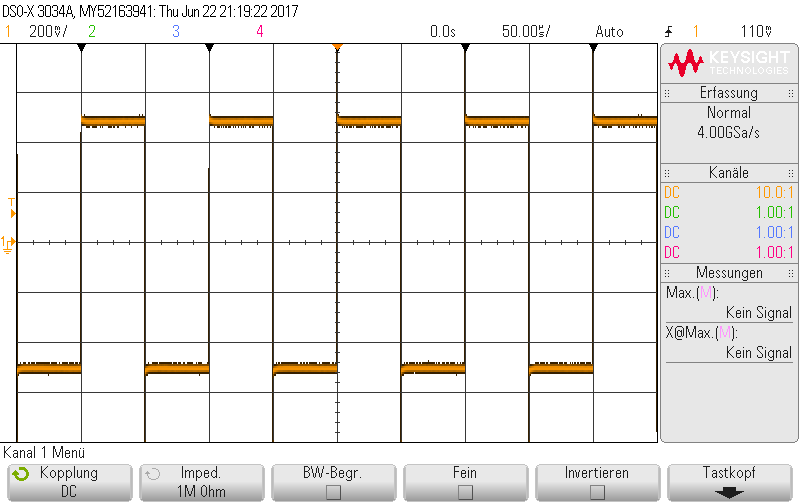
\includegraphics[height=3cm,width=6cm]{OsziBilder/bsp2_time.png}
  \end{center}
  \caption{Messwerte $0,1V$ DC}
\end{figure}
\end{minipage}
\begin{minipage}{.5\textwidth}
\begin{figure}[H]
  \begin{center}
   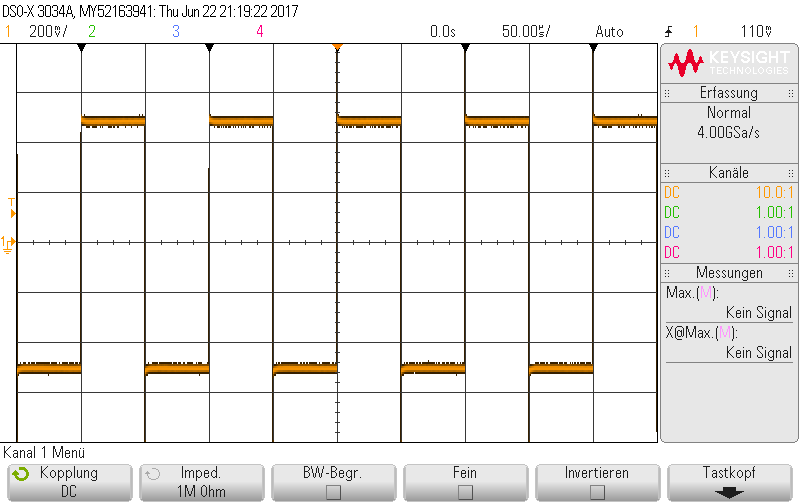
\includegraphics[height=3cm,width=6cm]{OsziBilder/bsp2_time.png}
  \end{center}
   \caption{Messwerte $0,3V$ DC}
\end{figure}
\end{minipage}
\end{table}
